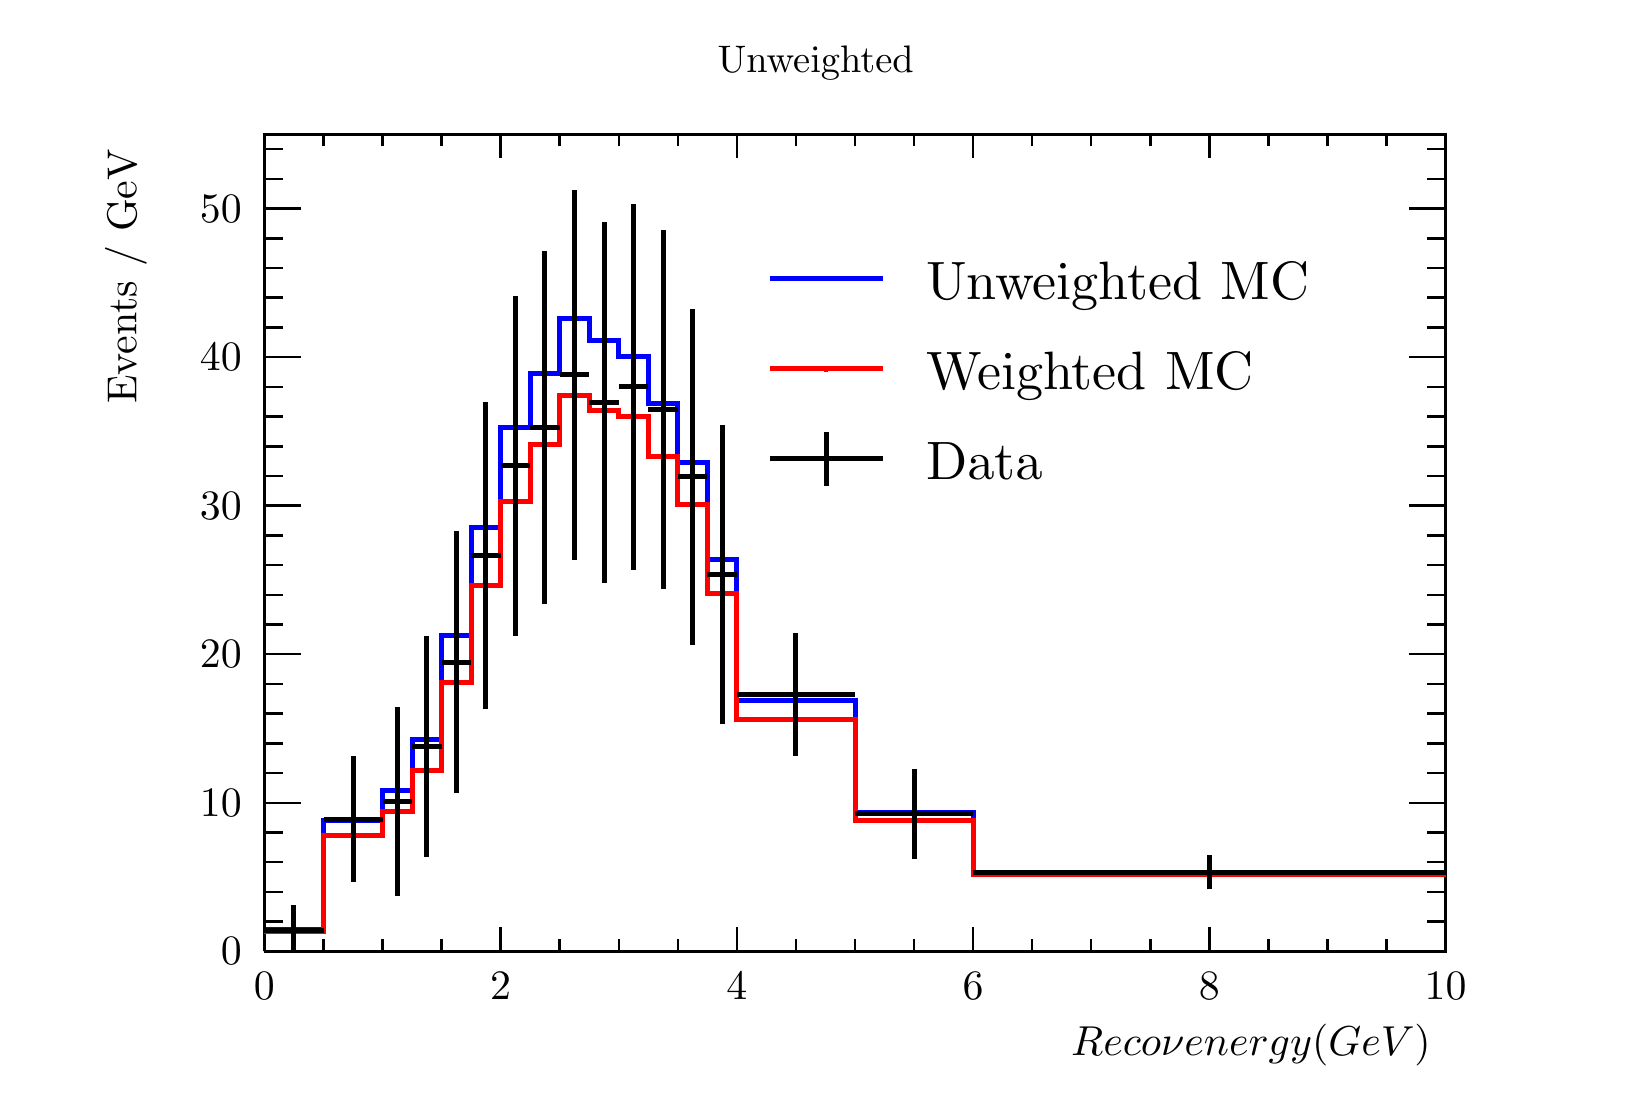
\begin{tikzpicture}
\pgfdeclareplotmark{cross} {
\pgfpathmoveto{\pgfpoint{-0.3\pgfplotmarksize}{\pgfplotmarksize}}
\pgfpathlineto{\pgfpoint{+0.3\pgfplotmarksize}{\pgfplotmarksize}}
\pgfpathlineto{\pgfpoint{+0.3\pgfplotmarksize}{0.3\pgfplotmarksize}}
\pgfpathlineto{\pgfpoint{+1\pgfplotmarksize}{0.3\pgfplotmarksize}}
\pgfpathlineto{\pgfpoint{+1\pgfplotmarksize}{-0.3\pgfplotmarksize}}
\pgfpathlineto{\pgfpoint{+0.3\pgfplotmarksize}{-0.3\pgfplotmarksize}}
\pgfpathlineto{\pgfpoint{+0.3\pgfplotmarksize}{-1.\pgfplotmarksize}}
\pgfpathlineto{\pgfpoint{-0.3\pgfplotmarksize}{-1.\pgfplotmarksize}}
\pgfpathlineto{\pgfpoint{-0.3\pgfplotmarksize}{-0.3\pgfplotmarksize}}
\pgfpathlineto{\pgfpoint{-1.\pgfplotmarksize}{-0.3\pgfplotmarksize}}
\pgfpathlineto{\pgfpoint{-1.\pgfplotmarksize}{0.3\pgfplotmarksize}}
\pgfpathlineto{\pgfpoint{-0.3\pgfplotmarksize}{0.3\pgfplotmarksize}}
\pgfpathclose
\pgfusepathqstroke
}
\pgfdeclareplotmark{cross*} {
\pgfpathmoveto{\pgfpoint{-0.3\pgfplotmarksize}{\pgfplotmarksize}}
\pgfpathlineto{\pgfpoint{+0.3\pgfplotmarksize}{\pgfplotmarksize}}
\pgfpathlineto{\pgfpoint{+0.3\pgfplotmarksize}{0.3\pgfplotmarksize}}
\pgfpathlineto{\pgfpoint{+1\pgfplotmarksize}{0.3\pgfplotmarksize}}
\pgfpathlineto{\pgfpoint{+1\pgfplotmarksize}{-0.3\pgfplotmarksize}}
\pgfpathlineto{\pgfpoint{+0.3\pgfplotmarksize}{-0.3\pgfplotmarksize}}
\pgfpathlineto{\pgfpoint{+0.3\pgfplotmarksize}{-1.\pgfplotmarksize}}
\pgfpathlineto{\pgfpoint{-0.3\pgfplotmarksize}{-1.\pgfplotmarksize}}
\pgfpathlineto{\pgfpoint{-0.3\pgfplotmarksize}{-0.3\pgfplotmarksize}}
\pgfpathlineto{\pgfpoint{-1.\pgfplotmarksize}{-0.3\pgfplotmarksize}}
\pgfpathlineto{\pgfpoint{-1.\pgfplotmarksize}{0.3\pgfplotmarksize}}
\pgfpathlineto{\pgfpoint{-0.3\pgfplotmarksize}{0.3\pgfplotmarksize}}
\pgfpathclose
\pgfusepathqfillstroke
}
\pgfdeclareplotmark{newstar} {
\pgfpathmoveto{\pgfqpoint{0pt}{\pgfplotmarksize}}
\pgfpathlineto{\pgfqpointpolar{44}{0.5\pgfplotmarksize}}
\pgfpathlineto{\pgfqpointpolar{18}{\pgfplotmarksize}}
\pgfpathlineto{\pgfqpointpolar{-20}{0.5\pgfplotmarksize}}
\pgfpathlineto{\pgfqpointpolar{-54}{\pgfplotmarksize}}
\pgfpathlineto{\pgfqpointpolar{-90}{0.5\pgfplotmarksize}}
\pgfpathlineto{\pgfqpointpolar{234}{\pgfplotmarksize}}
\pgfpathlineto{\pgfqpointpolar{198}{0.5\pgfplotmarksize}}
\pgfpathlineto{\pgfqpointpolar{162}{\pgfplotmarksize}}
\pgfpathlineto{\pgfqpointpolar{134}{0.5\pgfplotmarksize}}
\pgfpathclose
\pgfusepathqstroke
}
\pgfdeclareplotmark{newstar*} {
\pgfpathmoveto{\pgfqpoint{0pt}{\pgfplotmarksize}}
\pgfpathlineto{\pgfqpointpolar{44}{0.5\pgfplotmarksize}}
\pgfpathlineto{\pgfqpointpolar{18}{\pgfplotmarksize}}
\pgfpathlineto{\pgfqpointpolar{-20}{0.5\pgfplotmarksize}}
\pgfpathlineto{\pgfqpointpolar{-54}{\pgfplotmarksize}}
\pgfpathlineto{\pgfqpointpolar{-90}{0.5\pgfplotmarksize}}
\pgfpathlineto{\pgfqpointpolar{234}{\pgfplotmarksize}}
\pgfpathlineto{\pgfqpointpolar{198}{0.5\pgfplotmarksize}}
\pgfpathlineto{\pgfqpointpolar{162}{\pgfplotmarksize}}
\pgfpathlineto{\pgfqpointpolar{134}{0.5\pgfplotmarksize}}
\pgfpathclose
\pgfusepathqfillstroke
}
\definecolor{c}{rgb}{1,1,1};
\draw [color=c, fill=c] (0,0) rectangle (20,13.4752);
\draw [color=c, fill=c] (3,1.75177) rectangle (18,12.1277);
\definecolor{c}{rgb}{0,0,0};
\draw [c,line width=0.9] (3,1.75177) -- (3,12.1277) -- (18,12.1277) -- (18,1.75177) -- (3,1.75177);
\definecolor{c}{rgb}{1,1,1};
\draw [color=c, fill=c] (3,1.75177) rectangle (18,12.1277);
\definecolor{c}{rgb}{0,0,0};
\draw [c,line width=0.9] (3,1.75177) -- (3,12.1277) -- (18,12.1277) -- (18,1.75177) -- (3,1.75177);
\definecolor{c}{rgb}{0,0,1};
\draw [c,line width=1.8] (3,2.02999) -- (3.75,2.02999) -- (3.75,3.41537) -- (4.5,3.41537) -- (4.5,3.78866) -- (4.875,3.78866) -- (4.875,4.44674) -- (5.25,4.44674) -- (5.25,5.766) -- (5.625,5.766) -- (5.625,7.13898) -- (6,7.13898) -- (6,8.39894) --
 (6.375,8.39894) -- (6.375,9.08605) -- (6.75,9.08605) -- (6.75,9.7944) -- (7.125,9.7944) -- (7.125,9.50358) -- (7.5,9.50358) -- (7.5,9.31055) -- (7.875,9.31055) -- (7.875,8.7104) -- (8.25,8.7104) -- (8.25,7.96606) -- (8.625,7.96606) --
 (8.625,6.72203) -- (9,6.72203) -- (9,4.93791) -- (10.5,4.93791) -- (10.5,3.51015) -- (12,3.51015) -- (12,2.74254) -- (18,2.74254);
\definecolor{c}{rgb}{0,0,0};
\draw [c,line width=0.9] (3,1.75177) -- (18,1.75177);
\draw [c,line width=0.9] (3,2.05496) -- (3,1.75177);
\draw [c,line width=0.9] (3.75,1.90337) -- (3.75,1.75177);
\draw [c,line width=0.9] (4.5,1.90337) -- (4.5,1.75177);
\draw [c,line width=0.9] (5.25,1.90337) -- (5.25,1.75177);
\draw [c,line width=0.9] (6,2.05496) -- (6,1.75177);
\draw [c,line width=0.9] (6.75,1.90337) -- (6.75,1.75177);
\draw [c,line width=0.9] (7.5,1.90337) -- (7.5,1.75177);
\draw [c,line width=0.9] (8.25,1.90337) -- (8.25,1.75177);
\draw [c,line width=0.9] (9,2.05496) -- (9,1.75177);
\draw [c,line width=0.9] (9.75,1.90337) -- (9.75,1.75177);
\draw [c,line width=0.9] (10.5,1.90337) -- (10.5,1.75177);
\draw [c,line width=0.9] (11.25,1.90337) -- (11.25,1.75177);
\draw [c,line width=0.9] (12,2.05496) -- (12,1.75177);
\draw [c,line width=0.9] (12.75,1.90337) -- (12.75,1.75177);
\draw [c,line width=0.9] (13.5,1.90337) -- (13.5,1.75177);
\draw [c,line width=0.9] (14.25,1.90337) -- (14.25,1.75177);
\draw [c,line width=0.9] (15,2.05496) -- (15,1.75177);
\draw [c,line width=0.9] (15.75,1.90337) -- (15.75,1.75177);
\draw [c,line width=0.9] (16.5,1.90337) -- (16.5,1.75177);
\draw [c,line width=0.9] (17.25,1.90337) -- (17.25,1.75177);
\draw [c,line width=0.9] (18,2.05496) -- (18,1.75177);
\draw [anchor=base] (3,1.14539) node[scale=1.51215, color=c, rotate=0]{0};
\draw [anchor=base] (6,1.14539) node[scale=1.51215, color=c, rotate=0]{2};
\draw [anchor=base] (9,1.14539) node[scale=1.51215, color=c, rotate=0]{4};
\draw [anchor=base] (12,1.14539) node[scale=1.51215, color=c, rotate=0]{6};
\draw [anchor=base] (15,1.14539) node[scale=1.51215, color=c, rotate=0]{8};
\draw [anchor=base] (18,1.14539) node[scale=1.51215, color=c, rotate=0]{10};
\draw [anchor= east] (18,0.565957) node[scale=1.51215, color=c, rotate=0]{$Reco \nu energy (GeV)$};
\draw [c,line width=0.9] (3,12.1277) -- (18,12.1277);
\draw [c,line width=0.9] (3,11.8245) -- (3,12.1277);
\draw [c,line width=0.9] (3.75,11.9761) -- (3.75,12.1277);
\draw [c,line width=0.9] (4.5,11.9761) -- (4.5,12.1277);
\draw [c,line width=0.9] (5.25,11.9761) -- (5.25,12.1277);
\draw [c,line width=0.9] (6,11.8245) -- (6,12.1277);
\draw [c,line width=0.9] (6.75,11.9761) -- (6.75,12.1277);
\draw [c,line width=0.9] (7.5,11.9761) -- (7.5,12.1277);
\draw [c,line width=0.9] (8.25,11.9761) -- (8.25,12.1277);
\draw [c,line width=0.9] (9,11.8245) -- (9,12.1277);
\draw [c,line width=0.9] (9.75,11.9761) -- (9.75,12.1277);
\draw [c,line width=0.9] (10.5,11.9761) -- (10.5,12.1277);
\draw [c,line width=0.9] (11.25,11.9761) -- (11.25,12.1277);
\draw [c,line width=0.9] (12,11.8245) -- (12,12.1277);
\draw [c,line width=0.9] (12.75,11.9761) -- (12.75,12.1277);
\draw [c,line width=0.9] (13.5,11.9761) -- (13.5,12.1277);
\draw [c,line width=0.9] (14.25,11.9761) -- (14.25,12.1277);
\draw [c,line width=0.9] (15,11.8245) -- (15,12.1277);
\draw [c,line width=0.9] (15.75,11.9761) -- (15.75,12.1277);
\draw [c,line width=0.9] (16.5,11.9761) -- (16.5,12.1277);
\draw [c,line width=0.9] (17.25,11.9761) -- (17.25,12.1277);
\draw [c,line width=0.9] (18,11.8245) -- (18,12.1277);
\draw [c,line width=0.9] (3,1.75177) -- (3,12.1277);
\draw [c,line width=0.9] (3.462,1.75177) -- (3,1.75177);
\draw [c,line width=0.9] (3.231,2.12908) -- (3,2.12908);
\draw [c,line width=0.9] (3.231,2.50638) -- (3,2.50638);
\draw [c,line width=0.9] (3.231,2.88369) -- (3,2.88369);
\draw [c,line width=0.9] (3.231,3.26099) -- (3,3.26099);
\draw [c,line width=0.9] (3.462,3.6383) -- (3,3.6383);
\draw [c,line width=0.9] (3.231,4.0156) -- (3,4.0156);
\draw [c,line width=0.9] (3.231,4.39291) -- (3,4.39291);
\draw [c,line width=0.9] (3.231,4.77021) -- (3,4.77021);
\draw [c,line width=0.9] (3.231,5.14752) -- (3,5.14752);
\draw [c,line width=0.9] (3.462,5.52482) -- (3,5.52482);
\draw [c,line width=0.9] (3.231,5.90213) -- (3,5.90213);
\draw [c,line width=0.9] (3.231,6.27943) -- (3,6.27943);
\draw [c,line width=0.9] (3.231,6.65674) -- (3,6.65674);
\draw [c,line width=0.9] (3.231,7.03404) -- (3,7.03404);
\draw [c,line width=0.9] (3.462,7.41135) -- (3,7.41135);
\draw [c,line width=0.9] (3.231,7.78865) -- (3,7.78865);
\draw [c,line width=0.9] (3.231,8.16596) -- (3,8.16596);
\draw [c,line width=0.9] (3.231,8.54326) -- (3,8.54326);
\draw [c,line width=0.9] (3.231,8.92057) -- (3,8.92057);
\draw [c,line width=0.9] (3.462,9.29787) -- (3,9.29787);
\draw [c,line width=0.9] (3.231,9.67518) -- (3,9.67518);
\draw [c,line width=0.9] (3.231,10.0525) -- (3,10.0525);
\draw [c,line width=0.9] (3.231,10.4298) -- (3,10.4298);
\draw [c,line width=0.9] (3.231,10.8071) -- (3,10.8071);
\draw [c,line width=0.9] (3.462,11.1844) -- (3,11.1844);
\draw [c,line width=0.9] (3.462,11.1844) -- (3,11.1844);
\draw [c,line width=0.9] (3.231,11.5617) -- (3,11.5617);
\draw [c,line width=0.9] (3.231,11.939) -- (3,11.939);
\draw [anchor= east] (2.9,1.75177) node[scale=1.51215, color=c, rotate=0]{0};
\draw [anchor= east] (2.9,3.6383) node[scale=1.51215, color=c, rotate=0]{10};
\draw [anchor= east] (2.9,5.52482) node[scale=1.51215, color=c, rotate=0]{20};
\draw [anchor= east] (2.9,7.41135) node[scale=1.51215, color=c, rotate=0]{30};
\draw [anchor= east] (2.9,9.29787) node[scale=1.51215, color=c, rotate=0]{40};
\draw [anchor= east] (2.9,11.1844) node[scale=1.51215, color=c, rotate=0]{50};
\draw [anchor= east] (1.24,12.1277) node[scale=1.51215, color=c, rotate=90]{Events / GeV};
\draw [c,line width=0.9] (18,1.75177) -- (18,12.1277);
\draw [c,line width=0.9] (17.538,1.75177) -- (18,1.75177);
\draw [c,line width=0.9] (17.769,2.12908) -- (18,2.12908);
\draw [c,line width=0.9] (17.769,2.50638) -- (18,2.50638);
\draw [c,line width=0.9] (17.769,2.88369) -- (18,2.88369);
\draw [c,line width=0.9] (17.769,3.26099) -- (18,3.26099);
\draw [c,line width=0.9] (17.538,3.6383) -- (18,3.6383);
\draw [c,line width=0.9] (17.769,4.0156) -- (18,4.0156);
\draw [c,line width=0.9] (17.769,4.39291) -- (18,4.39291);
\draw [c,line width=0.9] (17.769,4.77021) -- (18,4.77021);
\draw [c,line width=0.9] (17.769,5.14752) -- (18,5.14752);
\draw [c,line width=0.9] (17.538,5.52482) -- (18,5.52482);
\draw [c,line width=0.9] (17.769,5.90213) -- (18,5.90213);
\draw [c,line width=0.9] (17.769,6.27943) -- (18,6.27943);
\draw [c,line width=0.9] (17.769,6.65674) -- (18,6.65674);
\draw [c,line width=0.9] (17.769,7.03404) -- (18,7.03404);
\draw [c,line width=0.9] (17.538,7.41135) -- (18,7.41135);
\draw [c,line width=0.9] (17.769,7.78865) -- (18,7.78865);
\draw [c,line width=0.9] (17.769,8.16596) -- (18,8.16596);
\draw [c,line width=0.9] (17.769,8.54326) -- (18,8.54326);
\draw [c,line width=0.9] (17.769,8.92057) -- (18,8.92057);
\draw [c,line width=0.9] (17.538,9.29787) -- (18,9.29787);
\draw [c,line width=0.9] (17.769,9.67518) -- (18,9.67518);
\draw [c,line width=0.9] (17.769,10.0525) -- (18,10.0525);
\draw [c,line width=0.9] (17.769,10.4298) -- (18,10.4298);
\draw [c,line width=0.9] (17.769,10.8071) -- (18,10.8071);
\draw [c,line width=0.9] (17.538,11.1844) -- (18,11.1844);
\draw [c,line width=0.9] (17.538,11.1844) -- (18,11.1844);
\draw [c,line width=0.9] (17.769,11.5617) -- (18,11.5617);
\draw [c,line width=0.9] (17.769,11.939) -- (18,11.939);
\definecolor{c}{rgb}{1,1,1};
\draw [color=c, fill=c] (2,12.6667) rectangle (18,13.4078);
\definecolor{c}{rgb}{0,0,0};
\draw (10,13.0372) node[scale=1.38614, color=c, rotate=0]{Unweighted};
\definecolor{c}{rgb}{1,0,0};
\draw [c,line width=1.8] (3,2.00665) -- (3.75,2.00665) -- (3.75,3.2233) -- (4.5,3.2233) -- (4.5,3.52806) -- (4.875,3.52806) -- (4.875,4.05181) -- (5.25,4.05181) -- (5.25,5.16925) -- (5.625,5.16925) -- (5.625,6.39298) -- (6,6.39298) -- (6,7.46518) --
 (6.375,7.46518) -- (6.375,8.18436) -- (6.75,8.18436) -- (6.75,8.81487) -- (7.125,8.81487) -- (7.125,8.61643) -- (7.5,8.61643) -- (7.5,8.54439) -- (7.875,8.54439) -- (7.875,8.03468) -- (8.25,8.03468) -- (8.25,7.42528) -- (8.625,7.42528) --
 (8.625,6.2965) -- (9,6.2965) -- (9,4.69037) -- (10.5,4.69037) -- (10.5,3.4118) -- (12,3.4118) -- (12,2.72153) -- (18,2.72153);
\definecolor{c}{rgb}{0,0,0};
\draw [c,line width=1.8] (3.375,1.75177) -- (3.375,2.0196);
\draw [c,line width=1.8] (3.375,2.0196) -- (3.375,2.33748);
\draw [c,line width=1.8] (3,2.0196) -- (3.375,2.0196);
\draw [c,line width=1.8] (3.375,2.0196) -- (3.75,2.0196);
\foreach \P in {(3.375,2.0196)}{\draw[mark options={color=c,fill=c},mark size=2.402402pt, line width=0.000000pt, mark=*,mark size=1pt] plot coordinates {\P};}
\draw [c,line width=1.8] (4.125,2.63575) -- (4.125,3.43196);
\draw [c,line width=1.8] (4.125,3.43196) -- (4.125,4.22817);
\draw [c,line width=1.8] (3.75,3.43196) -- (4.125,3.43196);
\draw [c,line width=1.8] (4.125,3.43196) -- (4.5,3.43196);
\foreach \P in {(4.125,3.43196)}{\draw[mark options={color=c,fill=c},mark size=2.402402pt, line width=0.000000pt, mark=*,mark size=1pt] plot coordinates {\P};}
\draw [c,line width=1.8] (4.6875,2.45991) -- (4.6875,3.65985);
\draw [c,line width=1.8] (4.6875,3.65985) -- (4.6875,4.85978);
\draw [c,line width=1.8] (4.5,3.65985) -- (4.6875,3.65985);
\draw [c,line width=1.8] (4.6875,3.65985) -- (4.875,3.65985);
\foreach \P in {(4.6875,3.65985)}{\draw[mark options={color=c,fill=c},mark size=2.402402pt, line width=0.000000pt, mark=*,mark size=1pt] plot coordinates {\P};}
\draw [c,line width=1.8] (5.0625,2.95418) -- (5.0625,4.35604);
\draw [c,line width=1.8] (5.0625,4.35604) -- (5.0625,5.7579);
\draw [c,line width=1.8] (4.875,4.35604) -- (5.0625,4.35604);
\draw [c,line width=1.8] (5.0625,4.35604) -- (5.25,4.35604);
\foreach \P in {(5.0625,4.35604)}{\draw[mark options={color=c,fill=c},mark size=2.402402pt, line width=0.000000pt, mark=*,mark size=1pt] plot coordinates {\P};}
\draw [c,line width=1.8] (5.4375,3.75845) -- (5.4375,5.42285);
\draw [c,line width=1.8] (5.4375,5.42285) -- (5.4375,7.08725);
\draw [c,line width=1.8] (5.25,5.42285) -- (5.4375,5.42285);
\draw [c,line width=1.8] (5.4375,5.42285) -- (5.625,5.42285);
\foreach \P in {(5.4375,5.42285)}{\draw[mark options={color=c,fill=c},mark size=2.402402pt, line width=0.000000pt, mark=*,mark size=1pt] plot coordinates {\P};}
\draw [c,line width=1.8] (5.8125,4.82855) -- (5.8125,6.77561);
\draw [c,line width=1.8] (5.8125,6.77561) -- (5.8125,8.72267);
\draw [c,line width=1.8] (5.625,6.77561) -- (5.8125,6.77561);
\draw [c,line width=1.8] (5.8125,6.77561) -- (6,6.77561);
\foreach \P in {(5.8125,6.77561)}{\draw[mark options={color=c,fill=c},mark size=2.402402pt, line width=0.000000pt, mark=*,mark size=1pt] plot coordinates {\P};}
\draw [c,line width=1.8] (6.1875,5.76145) -- (6.1875,7.91867);
\draw [c,line width=1.8] (6.1875,7.91867) -- (6.1875,10.0759);
\draw [c,line width=1.8] (6,7.91867) -- (6.1875,7.91867);
\draw [c,line width=1.8] (6.1875,7.91867) -- (6.375,7.91867);
\foreach \P in {(6.1875,7.91867)}{\draw[mark options={color=c,fill=c},mark size=2.402402pt, line width=0.000000pt, mark=*,mark size=1pt] plot coordinates {\P};}
\draw [c,line width=1.8] (6.5625,6.16706) -- (6.5625,8.40828);
\draw [c,line width=1.8] (6.5625,8.40828) -- (6.5625,10.6495);
\draw [c,line width=1.8] (6.375,8.40828) -- (6.5625,8.40828);
\draw [c,line width=1.8] (6.5625,8.40828) -- (6.75,8.40828);
\foreach \P in {(6.5625,8.40828)}{\draw[mark options={color=c,fill=c},mark size=2.402402pt, line width=0.000000pt, mark=*,mark size=1pt] plot coordinates {\P};}
\draw [c,line width=1.8] (6.9375,6.72122) -- (6.9375,9.07142);
\draw [c,line width=1.8] (6.9375,9.07142) -- (6.9375,11.4216);
\draw [c,line width=1.8] (6.75,9.07142) -- (6.9375,9.07142);
\draw [c,line width=1.8] (6.9375,9.07142) -- (7.125,9.07142);
\foreach \P in {(6.9375,9.07142)}{\draw[mark options={color=c,fill=c},mark size=2.402402pt, line width=0.000000pt, mark=*,mark size=1pt] plot coordinates {\P};}
\draw [c,line width=1.8] (7.3125,6.42759) -- (7.3125,8.72083);
\draw [c,line width=1.8] (7.3125,8.72083) -- (7.3125,11.0141);
\draw [c,line width=1.8] (7.125,8.72083) -- (7.3125,8.72083);
\draw [c,line width=1.8] (7.3125,8.72083) -- (7.5,8.72083);
\foreach \P in {(7.3125,8.72083)}{\draw[mark options={color=c,fill=c},mark size=2.402402pt, line width=0.000000pt, mark=*,mark size=1pt] plot coordinates {\P};}
\draw [c,line width=1.8] (7.6875,6.5962) -- (7.6875,8.92236);
\draw [c,line width=1.8] (7.6875,8.92236) -- (7.6875,11.2485);
\draw [c,line width=1.8] (7.5,8.92236) -- (7.6875,8.92236);
\draw [c,line width=1.8] (7.6875,8.92236) -- (7.875,8.92236);
\foreach \P in {(7.6875,8.92236)}{\draw[mark options={color=c,fill=c},mark size=2.402402pt, line width=0.000000pt, mark=*,mark size=1pt] plot coordinates {\P};}
\draw [c,line width=1.8] (8.0625,6.35619) -- (8.0625,8.63531);
\draw [c,line width=1.8] (8.0625,8.63531) -- (8.0625,10.9144);
\draw [c,line width=1.8] (7.875,8.63531) -- (8.0625,8.63531);
\draw [c,line width=1.8] (8.0625,8.63531) -- (8.25,8.63531);
\foreach \P in {(8.0625,8.63531)}{\draw[mark options={color=c,fill=c},mark size=2.402402pt, line width=0.000000pt, mark=*,mark size=1pt] plot coordinates {\P};}
\draw [c,line width=1.8] (8.4375,5.64734) -- (8.4375,7.78021);
\draw [c,line width=1.8] (8.4375,7.78021) -- (8.4375,9.91307);
\draw [c,line width=1.8] (8.25,7.78021) -- (8.4375,7.78021);
\draw [c,line width=1.8] (8.4375,7.78021) -- (8.625,7.78021);
\foreach \P in {(8.4375,7.78021)}{\draw[mark options={color=c,fill=c},mark size=2.402402pt, line width=0.000000pt, mark=*,mark size=1pt] plot coordinates {\P};}
\draw [c,line width=1.8] (8.8125,4.63398) -- (8.8125,6.53355);
\draw [c,line width=1.8] (8.8125,6.53355) -- (8.8125,8.43312);
\draw [c,line width=1.8] (8.625,6.53355) -- (8.8125,6.53355);
\draw [c,line width=1.8] (8.8125,6.53355) -- (9,6.53355);
\foreach \P in {(8.8125,6.53355)}{\draw[mark options={color=c,fill=c},mark size=2.402402pt, line width=0.000000pt, mark=*,mark size=1pt] plot coordinates {\P};}
\draw [c,line width=1.8] (9.75,4.22812) -- (9.75,5.01243);
\draw [c,line width=1.8] (9.75,5.01243) -- (9.75,5.79673);
\draw [c,line width=1.8] (9,5.01243) -- (9.75,5.01243);
\draw [c,line width=1.8] (9.75,5.01243) -- (10.5,5.01243);
\foreach \P in {(9.75,5.01243)}{\draw[mark options={color=c,fill=c},mark size=2.402402pt, line width=0.000000pt, mark=*,mark size=1pt] plot coordinates {\P};}
\draw [c,line width=1.8] (11.25,2.92308) -- (11.25,3.49685);
\draw [c,line width=1.8] (11.25,3.49685) -- (11.25,4.07062);
\draw [c,line width=1.8] (10.5,3.49685) -- (11.25,3.49685);
\draw [c,line width=1.8] (11.25,3.49685) -- (12,3.49685);
\foreach \P in {(11.25,3.49685)}{\draw[mark options={color=c,fill=c},mark size=2.402402pt, line width=0.000000pt, mark=*,mark size=1pt] plot coordinates {\P};}
\draw [c,line width=1.8] (15,2.53815) -- (15,2.75575);
\draw [c,line width=1.8] (15,2.75575) -- (15,2.97335);
\draw [c,line width=1.8] (12,2.75575) -- (15,2.75575);
\draw [c,line width=1.8] (15,2.75575) -- (18,2.75575);
\foreach \P in {(15,2.75575)}{\draw[mark options={color=c,fill=c},mark size=2.402402pt, line width=0.000000pt, mark=*,mark size=1pt] plot coordinates {\P};}
\definecolor{c}{rgb}{1,1,1};
\draw [color=c, fill=c] (9.10638,7.43262) rectangle (17.3333,10.8652);
\definecolor{c}{rgb}{0,0,0};
\draw [anchor=base west] (11.1631,10.0357) node[scale=1.95319, color=c, rotate=0]{Unweighted MC};
\definecolor{c}{rgb}{0,0,1};
\draw [c,line width=1.8] (9.41489,10.2931) -- (10.8546,10.2931);
\definecolor{c}{rgb}{0,0,0};
\draw [anchor=base west] (11.1631,8.89149) node[scale=1.95319, color=c, rotate=0]{Weighted MC};
\definecolor{c}{rgb}{1,1,1};
\draw [c, fill=c] (9.41489,8.74846) -- (10.8546,8.74846) -- (10.8546,9.54941) -- (9.41489,9.54941);
\definecolor{c}{rgb}{1,0,0};
\draw [c,line width=1.8] (9.41489,9.14894) -- (10.8546,9.14894);
\foreach \P in {(10.1348,9.14894)}{\draw[mark options={color=c,fill=c},mark size=2.402402pt, line width=0.000000pt, mark=*,mark size=1pt] plot coordinates {\P};}
\definecolor{c}{rgb}{0,0,0};
\draw [anchor=base west] (11.1631,7.74728) node[scale=1.95319, color=c, rotate=0]{Data};
\draw [c,line width=1.8] (9.41489,8.00473) -- (10.8546,8.00473);
\draw [c,line width=1.8] (10.1348,7.66147) -- (10.1348,8.34799);
\end{tikzpicture}
